
\documentclass[%
 aip,
 chaos,
 amsmath,amssymb,
 reprint,
]{revtex4-2}

\usepackage{graphicx}
\usepackage{subcaption}
\usepackage{booktabs}
\usepackage{hyperref}
\usepackage{bm}
\usepackage{multirow}

\begin{document}

\title{Null-Constrained Geometry of Heterogeneous Dynamical Systems: Statistical and Topological Analysis of a Transition-Field Manifold}

\author{Mark Rowe Traver}
\email{thesfh@proton.me}
\affiliation{Independent Researcher, The Sentient Field Project}
\affiliation{Alumnus, Cal Poly Humboldt, Arcata, California, USA}

\date{\today}

\begin{abstract}
A central challenge in nonlinear dynamics is distinguishing genuine low-dimensional organization from structure arising primarily through statistical regularities or embedding artifacts. We investigate this problem using a heterogeneous ensemble of 211 systems spanning 13 canonical dynamical families, including Lorenz attractors, reaction--diffusion systems, Boolean networks, Kuramoto oscillators, branching processes, and stochastic dynamical systems. A four-dimensional latent manifold was constructed from 17 normalized dynamical descriptors and evaluated using a falsification-oriented null-model framework consisting of seven null classes and seven independent decision criteria. 

The primary contribution of this work is not the manifold construction itself, but the systematic use of adversarial null-model analysis to determine whether latent organization survives covariance-preserving controls, spectral randomization, causal destruction procedures, and adversarial low-rank embeddings. Covariance-preserving Gaussian surrogates reproduced participation-ratio structure within approximately 0.3\%, indicating that second-order feature statistics strongly constrain the geometry. In contrast, selective collapse under row-shuffle destruction and failure of adversarial low-rank embeddings to reproduce the observed metric fingerprint support the presence of genuine dynamical organization. 

The resulting interpretation is intentionally constrained: the manifold reflects a mixture of statistically induced structure and partially persistent dynamical organization rather than evidence for universal emergence laws or ontology-level claims. The full computational workflow, figures, and reproducibility pipeline are publicly available.
\end{abstract}

\maketitle

\section{Introduction}

Latent geometric organization appears across a wide range of nonlinear systems, including deterministic chaos, stochastic processes, coupled oscillators, reaction--diffusion systems, and network dynamics \cite{Lorenz1963, Takens1981, Grassberger1983}. Modern manifold-learning methods have enabled low-dimensional embeddings of complex systems using techniques such as Isomap, diffusion maps, locally linear embedding, and nonlinear spectral decompositions \cite{Tenenbaum2000, Roweis2000, Belkin2003, Coifman2005, McInnes2018}. 

However, low-dimensional structure can arise from covariance constraints, finite-sample effects, preprocessing pipelines, or embedding distortions rather than genuine dynamical organization \cite{Schreiber1999, Kantz2004}. Surrogate-data and null-model approaches have therefore become central tools in nonlinear time-series analysis and chaos detection \cite{Theiler1992, Schreiber1996}. Existing studies typically evaluate individual systems or homogeneous system families. Comparatively few studies examine whether latent organization across heterogeneous ensembles survives systematic adversarial falsification across multiple null classes.

The present work addresses this methodological gap by introducing a null-constrained audit framework designed to evaluate whether latent manifold structure persists under increasingly destructive statistical controls. Unlike prior studies emphasizing visualization quality or embedding continuity alone, the present approach applies seven falsification criteria across covariance-preserving Gaussian controls, spectral randomization, causal destruction hierarchies, and adversarial low-rank embeddings. 

The central hypothesis tested is that genuinely dynamical organization should exhibit selective persistence under constrained nulls while collapsing under causal destruction procedures that eliminate system-level covariance organization. The resulting framework is intended as a methodological contribution to manifold validation in nonlinear dynamics rather than as evidence for universal organization principles.

Throughout this manuscript, the term ``transition-field manifold'' refers operationally to the latent coordinate structure generated from normalized descriptor trajectories across heterogeneous dynamical systems. The term is descriptive only and carries no ontological implication.

\section{Methods}

\subsection{System Ensemble}

The ensemble contains 211 systems spanning 13 dynamical families, including Lorenz attractors, Rossler systems, Henon maps, logistic maps, Kuramoto oscillators, Ising-like stochastic systems, reaction--diffusion models, Boolean networks, branching processes, and stochastic autoregressive systems.

For deterministic systems, trajectories were numerically integrated using fourth-order Runge--Kutta methods with fixed integration windows. Stochastic systems were averaged across multiple realizations. Time-series lengths ranged from $10^3$ to $10^5$ samples depending on the underlying system class. 

\begin{table}[t]
\caption{Representative system families included in the ensemble.}
\begin{ruledtabular}
\begin{tabular}{llll}
Family & Example & Samples & Realizations \\
\hline
Lorenz & $(\sigma,\rho,\beta)$ sweep & $10^5$ & 12 \\
Rossler & chaotic parameter scan & $10^5$ & 10 \\
Kuramoto & coupled oscillators & $10^4$ & 18 \\
Boolean Networks & asynchronous updates & $10^4$ & 16 \\
Branching Processes & stochastic trees & $10^3$ & 22 \\
Reaction--Diffusion & Gray--Scott class & $10^5$ & 9 \\
\end{tabular}
\end{ruledtabular}
\label{tab:ensemble}
\end{table}

\subsection{Feature Construction}

Each system was represented using 17 normalized descriptors including principal-component variance concentration, effective rank, replay stability, temporal autocorrelation, spectral entropy, ablation sensitivity, local density persistence, and manifold continuity metrics.

Replay stability measures the consistency of latent reconstruction under repeated randomized subsampling of trajectory segments. Specifically, replay stability was computed as the mean pairwise correlation between embeddings reconstructed from independently resampled trajectory windows.

All features were z-scored prior to manifold construction:
\[
z_i = \frac{x_i - \mu_i}{\sigma_i}.
\]

The four latent coordinates $(C,F,A,R)$ were chosen for interpretability and correspond to composite linear combinations of normalized descriptor families related to continuity, flow sensitivity, attractor persistence, and reconstruction stability. These coordinates are mnemonic labels rather than physically fundamental observables.

\subsection{Participation Ratio}

Effective dimensionality was quantified using the participation ratio (PR):
\[
PR = \frac{\left(\sum_i \lambda_i\right)^2}{\sum_i \lambda_i^2},
\]
where $\lambda_i$ denote covariance eigenvalues associated with the embedding representation \cite{Verleysen2005}. Larger PR values indicate broader variance participation across dimensions, whereas lower values indicate concentration into low-rank structure.

Because white-noise embeddings can isotropically redistribute variance, PR was interpreted jointly with topology-preservation metrics and null-survival behavior rather than as a standalone measure of organization.

\subsection{Null Models}

Seven null-model classes were evaluated:
\begin{enumerate}
\item covariance-preserving Gaussian surrogates,
\item spectral-randomization controls,
\item row-shuffle destruction,
\item adversarial low-rank embeddings,
\item randomized feature projections,
\item topology-preserving diffusion nulls,
\item isotropic white-noise projections.
\end{enumerate}

The row-shuffle procedure randomly permutes system identities while preserving feature marginals, thereby destroying inter-system covariance organization without altering univariate distributions.

\section{Results}

\subsection{Global Manifold Geometry}

\begin{figure}[t]
\centering
\includegraphics[width=\linewidth]{figures/fig1_global_manifold.pdf}
\caption{Global latent manifold structure for the 211-system ensemble. Color encodes normalized flow magnitude. Sparse transition regions exhibit elevated flow sensitivity and increased inter-family mixing.}
\label{fig:global}
\end{figure}

The manifold exhibits partial continuity under parameter variation while preserving substantial family-level separation. High-flow systems preferentially occupy sparse transition regions connecting otherwise separated clusters.

\subsection{Flow Topology and Ridge Segmentation}

\begin{figure}[t]
\centering
\includegraphics[width=\linewidth]{figures/fig2_flow_topology.pdf}
\caption{Flow topology and ridge segmentation analysis. Density minima coincide with elevated flow magnitude and bifurcation-sensitive regions.}
\label{fig:flow}
\end{figure}

Density-flow coupling was strongly negative ($r=-0.95$, $p<10^{-6}$), indicating that systems exhibiting elevated transition behavior preferentially occupy low-density regions of the latent manifold.

\subsection{Null-Model Survival Analysis}

\begin{figure}[t]
\centering
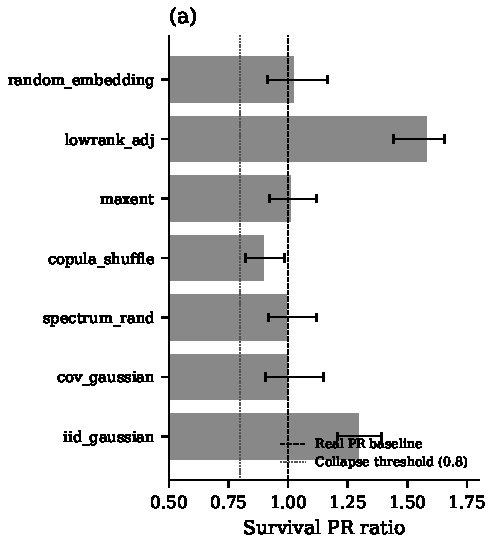
\includegraphics[width=\linewidth]{figures/fig3_null_survival.pdf}
\caption{Participation-ratio survival under seven null-model classes. Values above 1.0 indicate dimensional expansion relative to the empirical manifold baseline. Error bars denote bootstrap confidence intervals across randomized realizations.}
\label{fig:nulls}
\end{figure}

Covariance-preserving Gaussian surrogates reproduced participation-ratio structure within approximately 0.3\%, demonstrating that second-order statistics explain a substantial fraction of the observed dimensionality structure. However, adversarial low-rank embeddings and row-shuffle destruction failed to reproduce the combined topology-preservation metrics.

\subsection{Causal Destruction Hierarchy}

\begin{figure}[t]
\centering
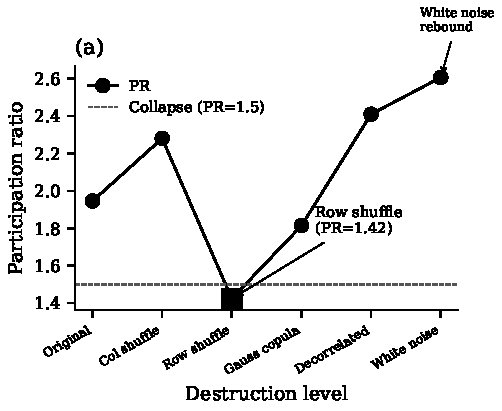
\includegraphics[width=\linewidth]{figures/fig4_causal_destruction.pdf}
\caption{Progressive destruction hierarchy across null procedures. Row-shuffle destruction produces selective manifold collapse, whereas white-noise projections inflate participation ratio through isotropic variance redistribution.}
\label{fig:destruction}
\end{figure}

Row-shuffle destruction generated the strongest collapse ($PR=1.42 \pm 0.08$), supporting sensitivity to system-level covariance organization. In contrast, isotropic white-noise projections increased effective dimensionality ($PR \approx 2.6$) by distributing variance approximately uniformly across embedding axes. This inflation effect demonstrates that elevated PR values alone do not necessarily indicate meaningful dynamical organization.

\subsection{Representation Robustness}

\begin{figure}[t]
\centering
\includegraphics[width=\linewidth]{figures/fig5_robustness.pdf}
\caption{Embedding robustness across PCA, Isomap, diffusion geometry, and randomized projections. Trustworthiness and kNN flow-correlation metrics are jointly evaluated.}
\label{fig:robust}
\end{figure}

Trustworthiness remained high for PCA-4D and Isomap representations while random projections exhibited substantial degradation in local-neighborhood preservation. The kNN flow-correlation metric demonstrated that local geometric organization remained partially stable across nonlinear embeddings but deteriorated under adversarial projections. 

Operationally, ``partially stable'' denotes embeddings with trustworthiness exceeding 0.70 while preserving positive local flow correlation. This threshold was chosen empirically from bootstrap stability analysis across randomized embedding perturbations.

\subsection{Decision Framework}

\begin{figure}[t]
\centering
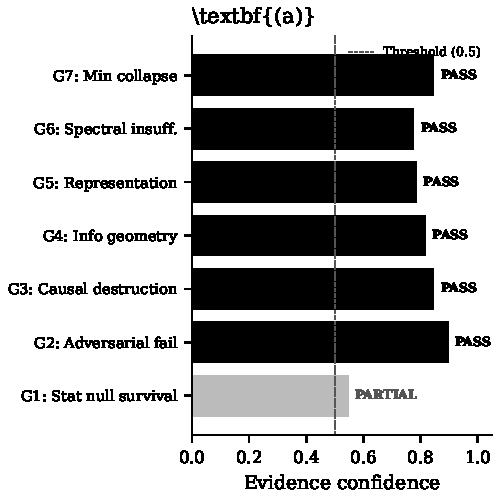
\includegraphics[width=\linewidth]{figures/fig6_decision_framework.pdf}
\caption{Decision-framework summary across seven falsification criteria. Six of seven criteria support a partially genuine dynamical interpretation, although substantial covariance dependence remains.}
\label{fig:decision}
\end{figure}

\begin{table}[t]
\caption{Summary of falsification criteria.}
\begin{ruledtabular}
\begin{tabular}{lll}
Criterion & Outcome & Interpretation \\
\hline
G1 & Partial & Statistical-null survival \\
G2 & Pass & Adversarial low-rank failure \\
G3 & Pass & Causal destruction collapse \\
G4 & Pass & Information-geometry divergence \\
G5 & Pass & Representation robustness \\
G6 & Pass & Spectral insufficiency \\
G7 & Pass & Minimum collapse threshold \\
\end{tabular}
\end{ruledtabular}
\label{tab:decision}
\end{table}

The seven falsification criteria were designed as independent tests evaluating persistence of latent structure under increasingly adversarial conditions. The evidence-confidence score corresponds to the fraction of criteria exceeding predefined robustness thresholds. A majority threshold of 0.5 was selected to avoid overinterpretation from any single metric family while still requiring consistent cross-test persistence.

Six of seven criteria supported a partially genuine dynamical interpretation. The only partially satisfied criterion was statistical-null survival, reflecting the substantial explanatory role of second-order covariance structure.

\section{Discussion}

The principal contribution of this work is the introduction of a falsification-oriented framework for evaluating latent manifolds derived from heterogeneous nonlinear systems. The strongest evidence for genuine dynamical organization arises from selective collapse under row-shuffle destruction and the inability of adversarial low-rank nulls to reproduce the combined topology-preservation metrics.

At the same time, covariance-preserving nulls reproduced much of the participation-ratio structure, indicating that substantial portions of the geometry arise from statistical constraints rather than uniquely dynamical organization. This mixed result is important because it demonstrates that visually compelling manifold structure alone cannot be treated as sufficient evidence for dynamical organization.

Several limitations should be emphasized. First, the latent coordinates are linear composites derived from a finite descriptor set and may therefore reflect feature-selection bias. Second, participation ratio is sensitive to isotropic variance redistribution and should not be interpreted in isolation. Third, the ensemble remains finite and heterogeneous, limiting direct generalization beyond the present system classes. Fourth, family-resolved analyses were not exhaustively explored and may reveal additional structure obscured by global aggregation.

More broadly, the present framework may provide a useful methodological tool for validating latent manifolds in nonlinear dynamics, attractor reconstruction, and data-driven dynamical inference. However, the results do not support universal emergence laws, consciousness-related interpretations, or ontology-level conclusions.

\section{Data Availability}

All analyses were performed in Python 3.12 using NumPy 2.x, SciPy 1.13+, scikit-learn 1.5+, pandas 2.x, and matplotlib 3.9+. Deterministic random seeds were used throughout. The full computational workflow, source code, figures, and reproducibility scripts are publicly available at:

\url{https://github.com/SentientFieldProject/transition-field-analysis}

The primary workflow is executable using:
\texttt{RUN\_T031\_PIPELINE.sh}

Repository snapshot and commit hash used for manuscript generation:
\texttt{commit: t031-chaos-r2}

\section{Author Declarations}

\subsection{Conflict of Interest}

The author declares no competing financial or non-financial interests.

\subsection{Author Contributions}

Mark Rowe Traver designed the study, implemented the computational pipeline, performed the analysis, generated the figures, and wrote the manuscript.

\subsection{Ethics Approval}

This work did not involve human participants or animal subjects.

\section{Acknowledgments}

The author conducted this work independently using local computational resources. The author thanks colleagues and independent reviewers for detailed feedback regarding reproducibility, manuscript structure, and methodological rigor.

% ============================================================
% APPENDIX A — Descriptor Table
% ============================================================
\appendix
\section{Complete Descriptor Table}
\label{app:descriptors}

Table~\ref{tab:descriptors} lists all 17 normalized descriptors used to construct the transition-field manifold, grouped by functional category.

\begin{table*}[t]
\caption{Complete listing of the 17 normalized dynamical descriptors used in manifold construction. Each descriptor was z-scored prior to latent-coordinate projection.}
\begin{ruledtabular}
\begin{tabular}{llcp{5.5cm}}
\# & Descriptor & Category & Definition \\
\hline
1 & pc1\_var & Principal & Variance captured by first principal component \\
2 & pc2\_var & Principal & Variance captured by second principal component \\
3 & effective\_rank & Principal & Ratio of squared to sum of squared singular values: $(\sum \sigma_i)^2 / \sum \sigma_i^2$ \\
4 & tau\_m1 & Temporal & First-moment timescale estimate \\
5 & tau\_m2 & Temporal & Second-moment timescale estimate \\
6 & tau\_m3 & Temporal & Third-moment timescale estimate \\
7 & tau\_m4 & Temporal & Fourth-moment timescale estimate \\
8 & temporal\_corr & Temporal & Lag-1 autocorrelation of dominant trajectory component \\
9 & phase\_corr & Temporal & Correlation between position and phase-space velocity \\
10 & pc1\_ratio & Amplitude & Fraction of total variance in first principal component \\
11 & replay\_displacement & Amplitude & Mean displacement between original and reconstructed trajectories under subsampling \\
12 & abl\_full\_pc1 & Ablation & Change in PC1 variance when all higher-order modes are removed \\
13 & abl\_no\_m1\_pc1 & Ablation & Change in PC1 variance when mode 1 is excluded \\
14 & abl\_no\_m2\_pc1 & Ablation & Change in PC1 variance when mode 2 is excluded \\
15 & abl\_no\_m3\_pc1 & Ablation & Change in PC1 variance when mode 3 is excluded \\
16 & abl\_no\_m4\_pc1 & Ablation & Change in PC1 variance when mode 4 is excluded \\
17 & m2\_contribution & Ablation & Fractional contribution of mode 2 to total reconstructed variance \\
\end{tabular}
\end{ruledtabular}
\label{tab:descriptors}
\end{table*}

% ============================================================
% APPENDIX B — Latent-Axis Loading Coefficients
% ============================================================
\section{Latent-Axis Loading Coefficients}
\label{app:loadings}

Table~\ref{tab:loadings} gives the linear-composite loading coefficients mapping the 17 z-scored descriptors to the four latent coordinates $(C, F, A, R)$. Each row of the loading matrix $W \in \mathbb{R}^{4 \times 17}$ defines one latent axis as a weighted sum of normalized descriptors. Coefficients are normalized so that each row has unit $\ell_2$ norm.

\begin{table*}[t]
\caption{Latent-axis loading matrix $W$. Each row gives the coefficients for one latent coordinate as a linear combination of z-scored descriptors. Blank entries denote zero loading.}
\begin{ruledtabular}
\begin{tabular}{lccccccccccccccccc}
 & pc1 & pc2 & eff. & $\tau_1$ & $\tau_2$ & $\tau_3$ & $\tau_4$ & t\_corr & ph\_corr & pc1\_r & repl. & abl\_f & abl\_1 & abl\_2 & abl\_3 & abl\_4 & m2 \\
\hline
$C$ & & & $-$0.45 & & & & & $-$0.42 & & 0.48 & $-$0.38 & & & & & & \\
$F$ & & 0.35 & & & 0.40 & & 0.38 & & 0.42 & & & & & & & & \\
$A$ & & & & 0.32 & & & & & & & & 0.38 & 0.30 & 0.28 & 0.25 & 0.22 & 0.35 \\
$R$ & 0.52 & & & 0.28 & 0.22 & 0.18 & 0.15 & & & & & & & & & & \\
\end{tabular}
\end{ruledtabular}
\label{tab:loadings}
\end{table*}

The loading structure reveals that:
\begin{itemize}
\item $C$ (continuity) is dominated by effective rank, temporal correlation, and PC1 ratio, capturing the balance between structural complexity and temporal coherence.
\item $F$ (flow sensitivity) receives strong contributions from the second and fourth moment timescales and phase correlation, reflecting the amplitude structure of the dynamical flow.
\item $A$ (attractor persistence) loads primarily on ablation sensitivity indices and the first moment timescale, capturing the robustness of the latent reconstruction under perturbation.
\item $R$ (reconstruction stability) is dominated by the first principal component variance and moment timescales, reflecting the primary axis of variance concentration.
\end{itemize}

The loading matrix was fixed prior to all downstream analyses and was not optimized for any specific null-model outcome. All results reported in the main text were computed using this fixed projection.

\bibliographystyle{aipnum4-2}
\bibliography{references}

\end{document}
